\documentclass{article}
\usepackage{pgfplots}
\pgfplotsset{compat=1.16}
\begin{document}

\begin{figure}[htbp]
    \centering
    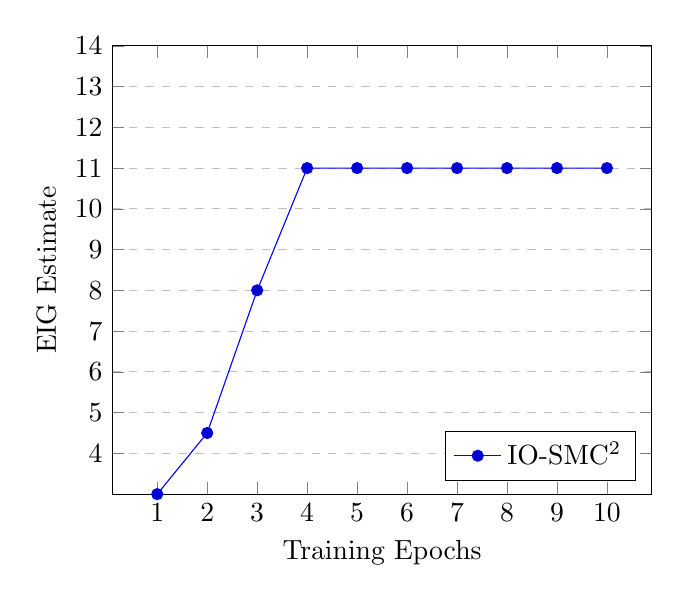
\begin{tikzpicture}
        \begin{axis}[
            xlabel={Training Epochs},
            ylabel={EIG Estimate},
            legend style={at={(0.97,0.03)},anchor=south east},
            ymajorgrids=true,
            grid style=dashed,
            error bars/y dir=both,
            error bars/y explicit,
            ymin=3,
            ymax=14,
            xtick={1,2,...,10},
            ytick={4,5,...,14},
            legend entries={IO-SMC$^2$},
            ]
            \addplot+[error bars/.cd,y dir=both, y explicit] coordinates {
                (1, 3) [y error={0.5}]
                (2, 4.5) [y error={0.5}]
                (3, 8) [y error={1.0}]
                (4, 11) [y error={1.0}]
                (5, 11) [y error={1.0}]
                (6, 11) [y error={1.0}]
                (7, 11) [y error={1.0}]
                (8, 11) [y error={1.0}]
                (9, 11) [y error={1.0}]
                (10, 11) [y error={1.0}]
            };
        \end{axis}
    \end{tikzpicture}
    \caption{Training evolution of the policy for the stochastic cart-pole experiment. We estimate the EIG after each training epoch, and we report the mean and standard deviation over 25 seeds.}
    \label{fig:training_eig}
\end{figure}

\end{document}